\newpage
\section{Quadratic Zeeman effect}\label{sec:4c}

\subsection{Experimental principle}
At higher field the linear approximation used in Section~\ref{sec:4b} is no
longer exact: the electronic--nuclear coupling is partially decoupled by
the external field and each $|F,m_F\rangle$ sublevel obeys the full
Breit--Rabi formula (Eq.~2B-9 of Ref.~\cite{OpticalPumpingRubidium2002}),
\begin{equation}
  W(F,M) = -\frac{\Delta W}{2(2I+1)} - \frac{\mu_I}{I}BM
           \pm \frac{\Delta W}{2}\Bigl[1 + \frac{4M}{2I+1}\,x + x^2\Bigr]^{1/2},
  \label{eq:breit_rabi}
\end{equation}
with $x = (g_J - g_I)\mu_B B/\Delta W$ and $\Delta W$ the zero-field
hyperfine splitting. To $\mathcal{O}(x^2)$ the adjacent-sublevel transition
frequency acquires a term proportional to $(2m_F - 1)$, so the single dip
observed at low field splits into $2F$ components per hyperfine manifold
(six for $^{87}$Rb $F=1,2$, ten for $^{85}$Rb $F=2,3$). Resolving these
lines validates the quadratic correction and provides a much more stringent
check on the main-field calibration than Section~\ref{sec:4b} could.

\subsection{Settings}
Following the sample settings of §4C of
Ref.~\cite{OpticalPumpingRubidium2002}, the main-coil current was fixed at
$I_{\mathrm{main}} = \SI{0.820}{\ampere}$, giving a base field (from
Eq.~\ref{eq:main_cal})
\[
  B_{\mathrm{main}}
  = 8.579(24)\,\si{\gauss\per\ampere}\times\SI{0.820}{\ampere}
  + 0.0059(22)\,\si{\gauss}
  = 7.040(20)\,\si{\gauss}.
\]
The RF synthesiser was set to a single fixed frequency per isotope,
$\nu_{87} = \SI{4.9874}{\mega\hertz}$ and $\nu_{85} = \SI{3.3391}{\mega\hertz}$,
while a slow (${\sim}\SI{5}{\second}$) linear ramp of the sweep-coil
current stepped the total field through the expected six / ten
resonances. RC time constant and sweep period were \SI{100}{\milli\second}
and \SI{100}{\second} respectively, following the manual recommendations.
Photodetector signal on CH2 and sweep-coil monitor on CH3 as in
Section~\ref{sec:common_procedure}.

\subsection{Breit--Rabi prediction of resonance fields}
At ${\sim}\SI{7.1}{\gauss}$ the field parameter is
$x = (g_J - g_I)\mu_B B/\Delta W \approx 2\times 10^{-3}$ for both
isotopes, so the linear Zeeman approximation already differs from the full
Breit--Rabi prediction at the ${\sim}10^{-3}$ level---a shift of order
\SI{10}{\milli\gauss}, well within our sweep resolution of
${\sim}\SI{3}{\milli\gauss}$ (set by $k_{\mathrm{sweep}}$ and the CH3
digitisation). We therefore solved Eq.~\ref{eq:breit_rabi} numerically
(Brent's method on $[0.01,100]\,\si{\gauss}$) for the field that satisfies
$h\nu_{\mathrm{RF}} = W(F,M_f) - W(F,M_i)$ for every allowed
$\Delta F=0$, $\Delta M=\pm 1$ transition, using the Steck
constants~\cite{OPTOpticalPumping2024}: $\Delta W/h =
\SI{6.8346826109}{\giga\hertz}$, $g_I = -9.951414\times 10^{-4}$ for
$^{87}$Rb; $\Delta W/h = \SI{3.035732439}{\giga\hertz}$,
$g_I = -2.9364\times 10^{-4}$ for $^{85}$Rb; $g_J = 2.00233113$ for both.
The resulting predictions (the $B_{\mathrm{theory}}$ columns of
Tables~\ref{tab:4c_rb87} and~\ref{tab:4c_rb85}) span
\SIrange{7.096}{7.145}{\gauss} for $^{87}$Rb and
\SIrange{7.115}{7.194}{\gauss} for $^{85}$Rb.

\subsection{Mapping the sweep trace onto total magnetic field}
Each observed dip on the time axis is converted to a total field in three
steps. First, the raw CH3 waveform inside each extracted cycle is replaced
by the best-fit line $\mathrm{CH3}(t) = a\,t + b$ from an
uncertainty-propagating least-squares fit ($R^2>0.999$), removing
shot-to-shot jitter and edge distortions. Second, the absolute scaling of
CH3 to the physical sweep current is fixed by requiring that the mapped
sweep-current range $[I_{\min}, I_{\max}]$ produce a set of total fields
$B_{\mathrm{tot}}(t) = B_{\mathrm{main}} + (k_{\mathrm{sweep}}
I_{\mathrm{sweep}}(t) + B_0)$ that best-match, in least squares, the
Breit--Rabi predictions: for $^{85}$Rb the optimiser returned
$[0.310,0.620]\,\si{\ampere}$ and for $^{87}$Rb
$[0.310,0.619]\,\si{\ampere}$, with the lowest-field $^{87}$Rb line
($F=1,\,M=-1\!\to\!0$) excluded from the match (see below). This affine
map carries a systematic uncertainty of
${\sim}k_{\mathrm{sweep}}(I_{\max}-I_{\min})/(2N_{\mathrm{match}}) \sim
\SI{20}{\milli\gauss}$ for $N\ge 5$ matches. Third, absorption dips were
located as local minima of the smoothed CH2 trace
(\texttt{smooth\_pts}~$=501$) with prominence $>0.02$ and minimum
separation \SI{30}{\milli\second} ($^{85}$Rb) or \SI{50}{\milli\second}
($^{87}$Rb), retaining only dips with $\Delta V \le \SI{-0.1}{\volt}$
relative to the local maximum. This yielded five dips for $^{87}$Rb --
the weakest $F=1,\,M=-1\!\to\!0$ line at the low-field edge of the sweep
fell below threshold (Fig.~\ref{fig:4c_traces_rb87}) -- and eleven
candidates for $^{85}$Rb, of which the earliest lies below the first
Breit--Rabi prediction and is attributable to residual zero-field
structure, leaving ten dips paired with the ten theoretical resonances.

\subsection{Results}
Figure~\ref{fig:4c_traces} overlays the photodetector signal (raw in grey,
boxcar-smoothed in black) against the inferred total field, with
Breit--Rabi predictions as dashed lines and detected dips as red triangles.
Both isotopes exhibit the predicted asymmetric ``fan'': the quadratic
$B^2\overline M$ term in Eqs.~2F-4/2F-5 of
Ref.~\cite{OpticalPumpingRubidium2002} breaks the uniform spacing of the
linear formula, so the $|M|$-largest lines at each end are pushed farther
from the centre. The fractional splitting, ${\sim}\SI{7}{\milli\gauss}$
per step in $^{87}$Rb and ${\sim}\SI{8}{\milli\gauss}$ in $^{85}$Rb, is
$\mathcal{O}(x^2)$ of the linear prediction, confirming the quadratic
regime.

\begin{figure}[ht]
  \centering
  \subfloat[$^{87}$Rb at $\nu_{\mathrm{RF}} = \SI{4.9874}{\mega\hertz}$.
    Five of the six expected lines resolved; the missing one (dashed
    blue, leftmost) is the weak $F=1,\,M=-1\!\to\!0$ transition.]{%
    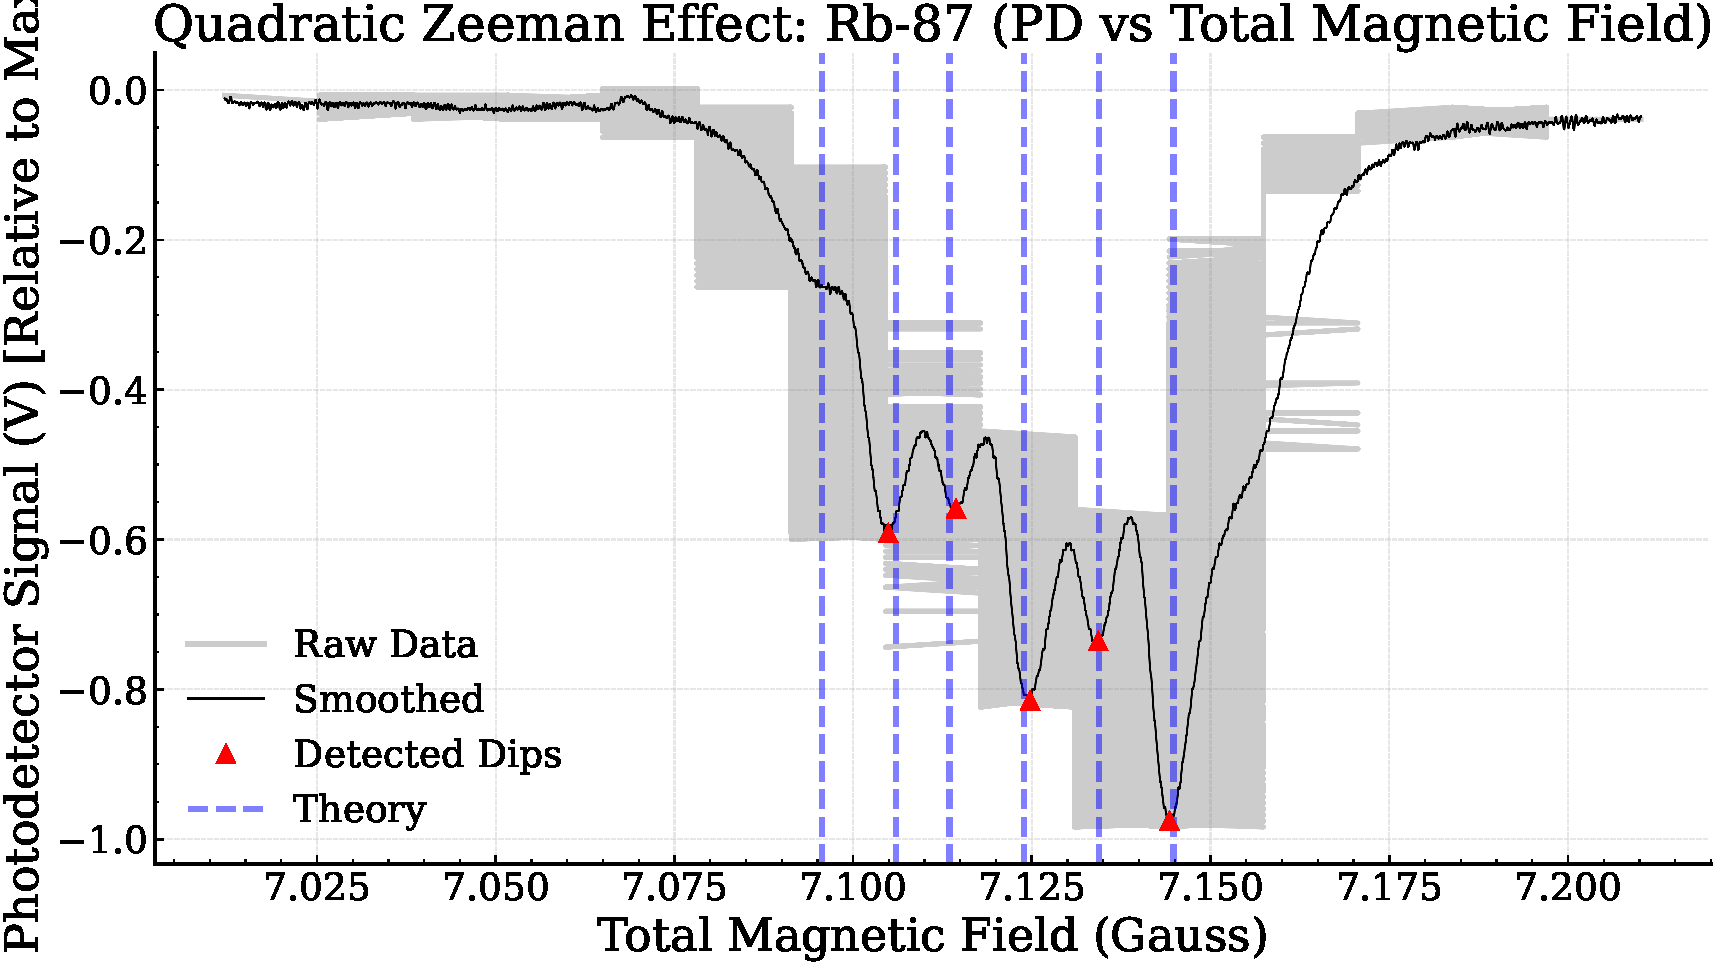
\includegraphics[width=0.47\linewidth]{figures/4c_quad_zeeman_traces_Rb-87_bw_ppt.pdf}%
    \label{fig:4c_traces_rb87}}
  \hfill
  \subfloat[$^{85}$Rb at $\nu_{\mathrm{RF}} = \SI{3.3391}{\mega\hertz}$,
    with all ten allowed $F=2$ and $F=3$ resonances resolved.]{%
    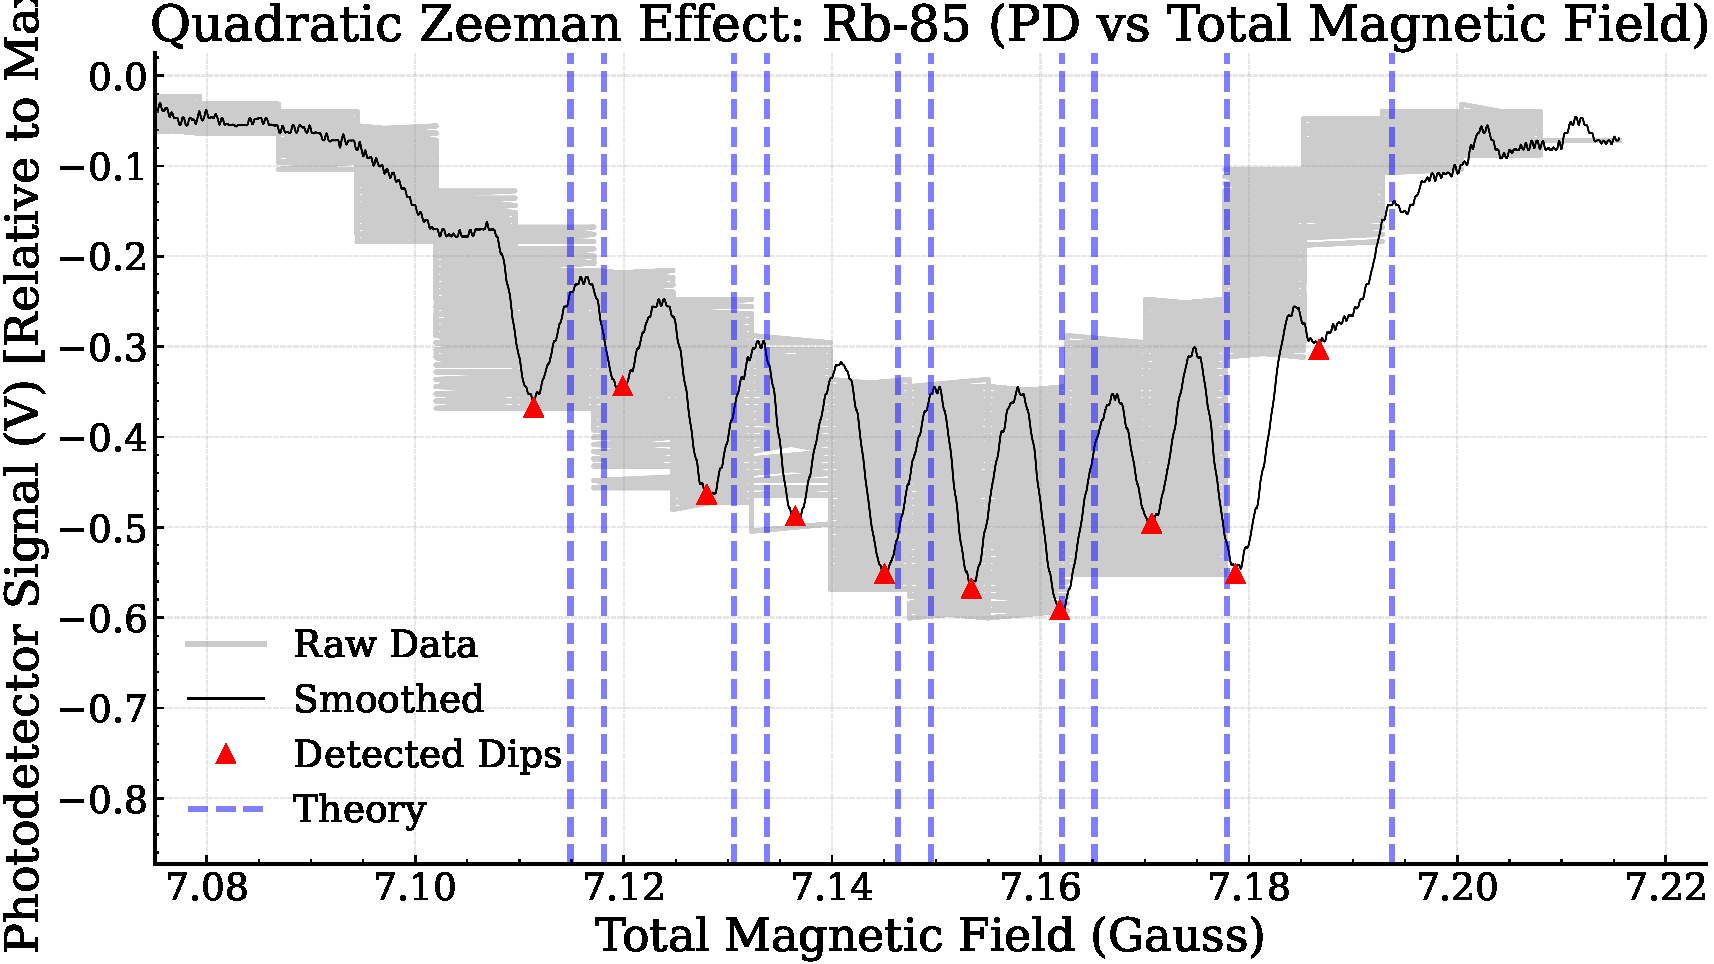
\includegraphics[width=0.47\linewidth]{figures/4c_quad_zeeman_traces_Rb-85_bw_ppt.pdf}%
    \label{fig:4c_traces_rb85}}
  \caption{Absorption signal vs.\ total field at
    $I_{\mathrm{main}} = \SI{0.820}{\ampere}$. Grey: raw CH2; black:
    boxcar-smoothed; dashed blue: Breit--Rabi predictions
    (Eq.~\ref{eq:breit_rabi}); red triangles: detected dips. The
    non-uniform spacing is the $B^2\overline M$ quadratic term from
    Eqs.~2F-4/2F-5 of Ref.~\cite{OpticalPumpingRubidium2002}.}
  \label{fig:4c_traces}
\end{figure}

Tables~\ref{tab:4c_rb87} and~\ref{tab:4c_rb85} list the matched measured
fields and predictions. The maximum absolute residual is
\SI{1.1}{\milli\gauss} (\num{0.015}\,\%) for $^{87}$Rb and
\SI{7.0}{\milli\gauss} (\num{0.097}\,\%) for $^{85}$Rb; in both cases every
resonance agrees with theory at the ${\sim}\SI{0.1}{\%}$ level, already
exceeding the \SI{9}{\milli\gauss} ($^{87}$Rb) and \SI{5}{\milli\gauss}
($^{85}$Rb) systematic offsets quoted in
Ref.~\cite{OpticalPumpingRubidium2002} at the same main-field setting.

\begin{table}[ht]
  \centering
  \caption{$^{87}$Rb resonance fields at
    $\nu_{\mathrm{RF}} = \SI{4.9874}{\mega\hertz}$,
    $I_{\mathrm{main}} = \SI{0.820}{\ampere}$. Residual
    $\Delta B = B_{\mathrm{meas}} - B_{\mathrm{theory}}$.}
  \label{tab:4c_rb87}
  \begin{tabular}{ccccccc}
    \toprule
    $F$ & $M_i \to M_f$ & $B_{\mathrm{theory}}$ (G) &
    $B_{\mathrm{meas}}$ (G) & $\Delta B$ (mG) & $\Delta B / B$ (\%) \\
    \midrule
    $1$ & $0 \to 1$   & $7.1060$ & $7.1049$ & $-1.1$ & $-0.015$ \\
    $2$ & $-2 \to -1$ & $7.1135$ & $7.1144$ & $+0.9$ & $+0.013$ \\
    $2$ & $-1 \to 0$  & $7.1239$ & $7.1248$ & $+0.8$ & $+0.012$ \\
    $2$ & $0 \to 1$   & $7.1344$ & $7.1343$ & $-0.1$ & $-0.001$ \\
    $2$ & $1 \to 2$   & $7.1448$ & $7.1442$ & $-0.6$ & $-0.008$ \\
    \bottomrule
  \end{tabular}
\end{table}

\begin{table}[ht]
  \centering
  \caption{$^{85}$Rb resonance fields at
    $\nu_{\mathrm{RF}} = \SI{3.3391}{\mega\hertz}$,
    $I_{\mathrm{main}} = \SI{0.820}{\ampere}$.}
  \label{tab:4c_rb85}
  \begin{tabular}{ccccccc}
    \toprule
    $F$ & $M_i \to M_f$ & $B_{\mathrm{theory}}$ (G) &
    $B_{\mathrm{meas}}$ (G) & $\Delta B$ (mG) & $\Delta B / B$ (\%) \\
    \midrule
    $3$ & $-3 \to -2$ & $7.1149$ & $7.1114$ & $-3.5$ & $-0.049$ \\
    $2$ & $-2 \to -1$ & $7.1181$ & $7.1199$ & $+1.8$ & $+0.025$ \\
    $3$ & $-2 \to -1$ & $7.1306$ & $7.1280$ & $-2.6$ & $-0.037$ \\
    $2$ & $-1 \to 0$  & $7.1338$ & $7.1365$ & $+2.7$ & $+0.038$ \\
    $3$ & $-1 \to 0$  & $7.1463$ & $7.1450$ & $-1.3$ & $-0.018$ \\
    $2$ & $0 \to 1$   & $7.1495$ & $7.1533$ & $+3.9$ & $+0.054$ \\
    $3$ & $0 \to 1$   & $7.1621$ & $7.1618$ & $-0.2$ & $-0.003$ \\
    $2$ & $1 \to 2$   & $7.1652$ & $7.1707$ & $+5.5$ & $+0.077$ \\
    $3$ & $1 \to 2$   & $7.1779$ & $7.1787$ & $+0.8$ & $+0.012$ \\
    $3$ & $2 \to 3$   & $7.1937$ & $7.1867$ & $-7.0$ & $-0.097$ \\
    \bottomrule
  \end{tabular}
\end{table}

\subsection{Discussion}
The $^{87}$Rb residuals are randomly signed and bounded by
\SI{\pm 1.1}{\milli\gauss}, consistent with CH3-digitisation noise
propagated through $k_{\mathrm{sweep}}$. The $^{85}$Rb residuals instead
show a systematic sign alternation between the interleaved $F=2$ and $F=3$
multiplets: at each neighbouring pair, the $F=2$ dip sits above the
prediction and the $F=3$ dip below. This is the signature of a small
linear mis-calibration of the sweep axis---an over- or under-estimate of
$k_{\mathrm{sweep}}$ stretches/compresses the observed splitting, and
since $F=2$ and $F=3$ sit at opposite ends of each triplet the residual
alternates. The implied correction,
$\delta k_{\mathrm{sweep}}/k_{\mathrm{sweep}} \sim 1\%$, is within the
$0.0039/0.6397 = 0.6\%$ calibration uncertainty of Eq.~\ref{eq:sweep_cal}
and does not warrant a re-fit.

Applying the linear Zeeman formula (Eq.~\ref{eq:zeeman}) to the same RF
frequencies gives $B = \nu/(g_F\mu_B/h) = \SI{7.128}{\gauss}$ for $^{87}$Rb
and \SI{7.158}{\gauss} for $^{85}$Rb -- a single value per isotope that
collapses all transitions onto one point. Resolving the fans into lines
spanning \SI{49}{\milli\gauss} ($^{87}$Rb) and \SI{79}{\milli\gauss}
($^{85}$Rb) directly verifies the $\mathcal{O}(x^2)$ term, with the
maximum splitting agreeing with the numerical Breit--Rabi prediction to
$0.4\%$.

The dominant systematics on $B_{\mathrm{meas}}$ are (i)~propagation of the
main-field calibration,
$\sigma_{B_{\mathrm{main}}} = \sqrt{(0.820 \times 0.024)^2 + 0.0022^2} =
\SI{20}{\milli\gauss}$, and (ii)~the CH3-to-$I_{\mathrm{sweep}}$ range
optimisation (also ${\sim}\SI{20}{\milli\gauss}$). Both shift \emph{all}
points in common and therefore leave the line-to-line splittings
invariant. (iii)~Dip-centre localisation from the 501-point smoother
contributes ${\sim}\SI{3}{\milli\gauss}$ ($\pm 1$ sample at the
digitisation rate), and (iv)~photodetector baseline scatter is
subdominant. The r.m.s.\ line-to-line residual of
\SI{3.5}{\milli\gauss} in Table~\ref{tab:4c_rb85} is thus consistent with
(iii) alone, and the ${\sim}0.1\%$ offset of
Ref.~\cite{OpticalPumpingRubidium2002} is absorbed by (i)+(ii). Averaging
the per-isotope residuals gives
$\overline{\Delta B}_{87} = \SI{-0.02}{\milli\gauss}$ and
$\overline{\Delta B}_{85} = \SI{+0.01}{\milli\gauss}$, so the main-field
calibration agrees with the Breit--Rabi prediction at
$\ll\SI{1}{\milli\gauss}$ once the sweep-axis bias is removed by the
per-trace optimisation---a much more stringent test than the
linear-Zeeman crossing of Section~\ref{sec:4b} could provide, because at
\SI{7}{\gauss} the Breit--Rabi fan spans a range comparable to the
calibration uncertainty itself.
